\documentclass{article}
\usepackage{graphicx}
\usepackage{amsmath}
\usepackage{hyperref}
\usepackage{float}
\usepackage{xcolor}
\usepackage{enumitem}
\usepackage{hyperref}
\usepackage{mathtools}

\begin{document}

\title{Solutions to hw3 homework on Convex Optimization https://web.stanford.edu/class/ee364b/homework.html}
\author{Andrei Keino}
\maketitle

\section*{3.1 (4 points)} 
Consider the optimization problem

\begin{align*}
	minimize_{\{x_j\}_{j = 1}^J} \; &  
	f(x_1, \dots, x_j) \coloneqq
	\frac{1}{2} \lVert b - \sum_{j = 1}^{J} 
	A_j x_j \rVert_2^2 
	+ \lambda \cdot   \sum_{j = 1}^{J} 
	\lVert x_j \rVert_2,
	\\
	& s.t. \; A_j x_j \geq 0, \; \forall j 
	\in \{1, 2, \dots, J\} \\
\end{align*}
with variable $x_1, \dots, x_J \in R^n, $ and 
problem data $A_1, \dots, A_J \in R^{m \times n}, $ 
$b \in R^m,$ and $\lambda > 0.$ for constrained optimization given on page 11 (really p. 12) of the lecture slides for subgradient methods for constrained problems. \\

% file 
% C:\! Convex_Optimization\ConvexOptimizationII\materials\lsocoee364b/03-constr_subgrad_slides.pdf

Let $J = 3,$ $n = 100,$ $m = 10$ and $\lambda = 0.5$ Generate random matrices
$A_1, \dots , A_J \in R^{m\times n}$ with independent uniformly distributed entries in the interval 
$[0, \frac{1}{\sqrt{m}}),$ and, random vectors $x_1, \dots,  x_J \in 2 R^n$uniformly distributed entries in the interval 
$[0, \frac{1}{\sqrt{n}}),$ then set 
$b = \sum_{j = 1}^{J} A_j x_j.$
Plot convergence in terms of the
objective $f(x_1^{(k)}, \dots x_1^{(J)}).$ 
Try different step length schedules. Also, plot the maximal violation for the linear constraints at each step.\\

Solution: \\
\textbf{The code is in the file} \verb |solution_3_1_b.m.| The code 
is nearly the same as one for the task 2.4, the only difference that on every step of the gradient descent we are calculating the constraint violation vector and if 
there are at least one violation, we replace the gradient of the minimized function with the gradient of any constraint violation found.

\begin{figure}[H]
	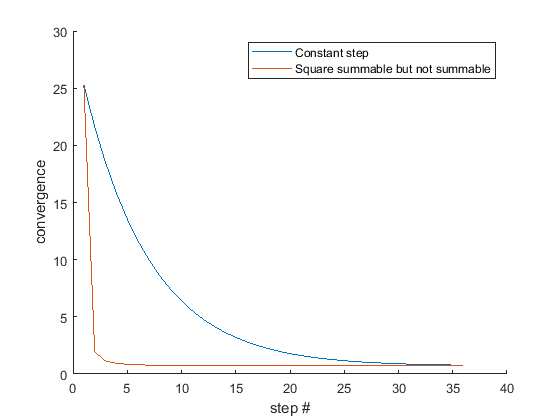
\includegraphics[width=\linewidth]{fig_3_1_1.png}
	\caption{Convergence with different step length.}
	\label{fig:3_1_1}
\end{figure}

\begin{figure}[H]
	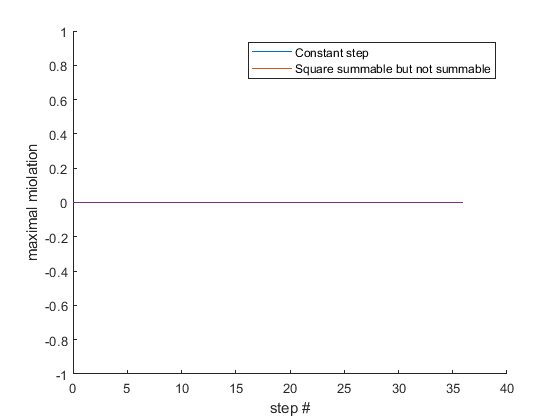
\includegraphics[width=\linewidth]{fig_3_1_2.png}
	\caption{Maximal violation for the linear constraints.}
	\label{fig:3_1_2}
\end{figure}






\end{document}